\section{The concrete design}\label{sec:design}

A design implementing the counter with $B=377$, $\nclocks$ clocks and $\nmoves$ taps was found by
computer search (Section~\ref{sec:search}):
\begin{center}\small
\begin{tabular}{ll}
\toprule
clocks $C$ & $1,2,3,4,19,28,29,40,63,91,92,124,126,127,128,145,163,191,217,231,$\\
 & $252,253,254,280,290,291,292,317,344,354$\\
wires $\rho$ & boot $0$, nm $5$, marker $18$, ncin $38$, nb $64$, $g_1$ $101$, carry $149$, $u$ $219$\\
\bottomrule
\end{tabular}
\end{center}
With $K=k-1$ the move set is $S_k=\{(aK+b)\cdot 377+\delta\}$ over the $\nmoves$ taps; explicitly
\begin{multline*}
S_k=\{5,7,8,13,20,30,31,43,47,50,55,66,69,70,76,77,80,83,85,111,118,136,138,\\
180,183,185,192,197,239,266,283,297,329,346,547\}\\
\cup\{377(k-1)+222,\ 377(k-1)+259,\ 377(k-1)+364\}.
\end{multline*}
The $35$ fixed moves are at most $547<377+222$, so the three $k$-dependent moves (the long delays
feeding nm, nb and $g_1$) are distinct from them and $|S_k|=\nmoves$ for all $k\ge2$, with
$\max S_k=377(k-1)+364=377k-13$.  Conditions \ref{c:K}--\ref{c:Z0} are finite and are verified
mechanically.  Figure~\ref{fig:bitmap} shows the resulting P-positions for $k=3$.

\begin{figure}[t]
\centering
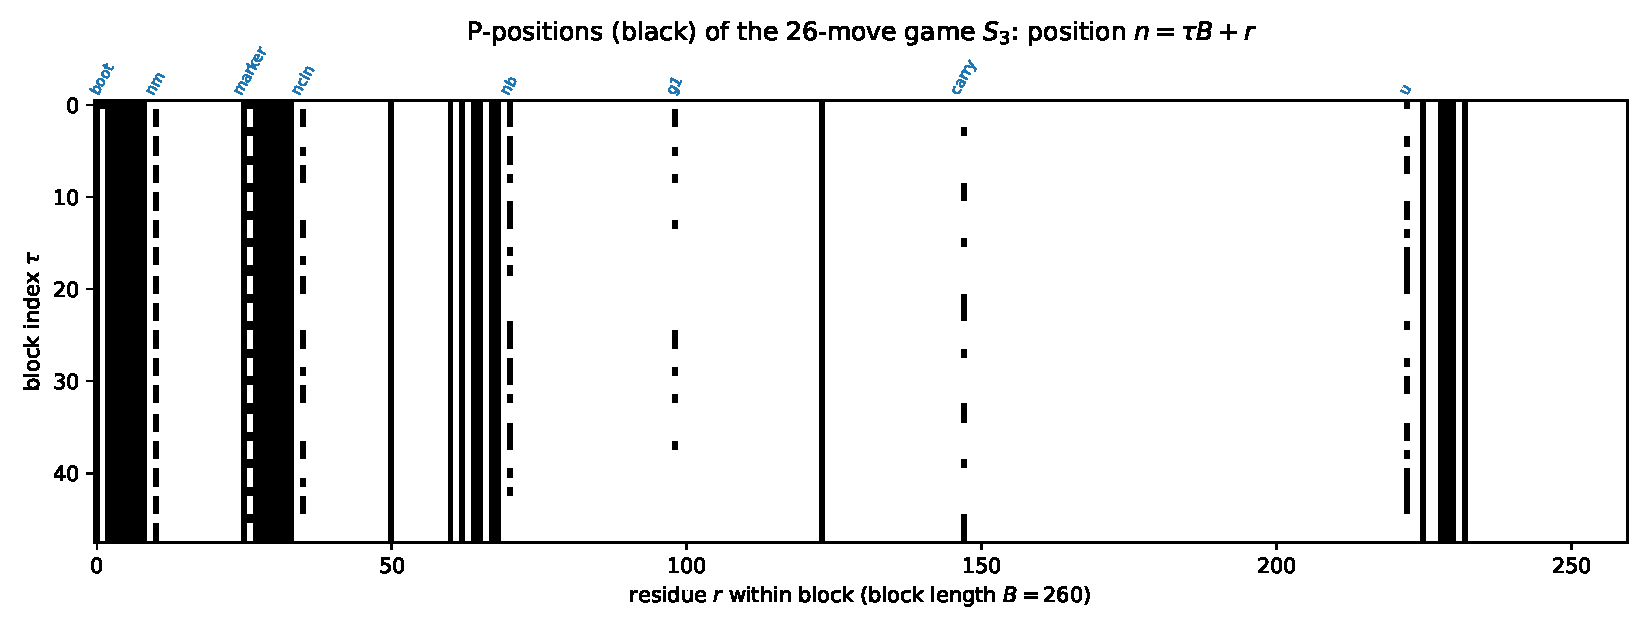
\includegraphics[width=\textwidth]{figs/bitmap.pdf}\\[2mm]
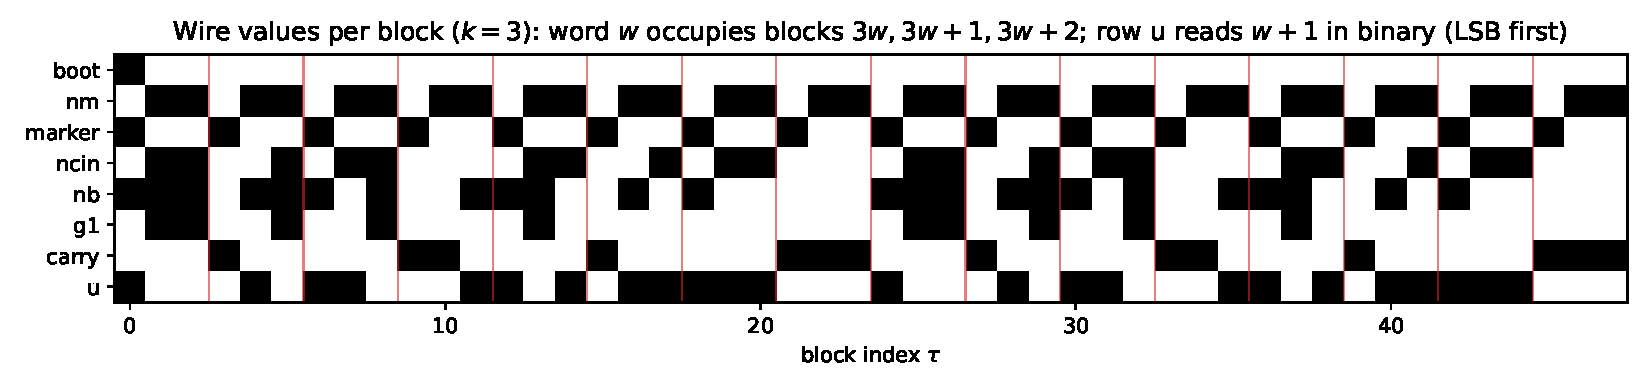
\includegraphics[width=\textwidth]{figs/wires.pdf}
\caption{Top: P-positions of the $\nmoves$-move game $S_3$, one block of $377$ positions per row.  Clocks
are the solid columns; the dashed columns are the eight wires.  Bottom: the wire values; the $u$ row
spells $1,2,3,\dots,7,0,1,\dots$ in binary, three blocks per word.  The period is
$377\cdot 3\cdot 2^3=9048$.}
\label{fig:bitmap}
\end{figure}

